\chapter{Magma Dynamics: porosity waves}
\label{cha:porosity-waves}

\section{Problem Overview}
\label{sec:porosity_waves-formulation}


While many modeling packages in Earth science solve for thermal or
thermo-chemical convection, one of the strengths of \TF{} is that it
is not a ``convection code'' or a ``lithosphere code'', but rather a
general finite element PDE solver that can be used to model arbitrary
problems as long as the weak forms are well posed.  In particular,
\TF{} was primarily designed to explore coupled fluid/solid mechanics
with a primary application area being the flow of magma and fluids in
the deep earth.  A more general theory of magma dynamics has been
derived by multiple authors
\cite{mckenzie_generation_1984,scott_magma_1984,scott_magma_1986,spiegelman_flow_1993,spiegelman_flow_1993-1,bercovici_two-phase_2001-1,bercovici_energetics_2003,simpson_multiscale_2010,simpson_multiscale_2010-1}
that considers the flow of a low viscosity fluid in a viscously
deformable solid matrix. This theory has been the basis for a large
number of models of magmatic regimes including mid-ocean ridges and
subduction zones.  However, rather than begin by developing such 
complex models,  it is useful to start with the basic benchmark
problems in magma-dynamics, namely calculating the evolution and
propagation of non-linear porosity waves.

From the beginning of magma dynamics, one of
the intriguing features of these equations is that they admit dispersive
non-linear magmatic solitary waves that propagate through the solid as
``hump shaped'' blobs with radial symmetry that propagate at a
characteristic speed $c$ that depends on amplitude, dimension and
material parameters.  Figure \ref{fig:SolitaryWavesAllD} shows some
example solitary wave profiles for 1,2 and 3-D solitary waves that all
propagate at the same speed $c=5$ times the melt velocity in the
background constant porosity region.

\begin{figure}[htb!]
  \centering
  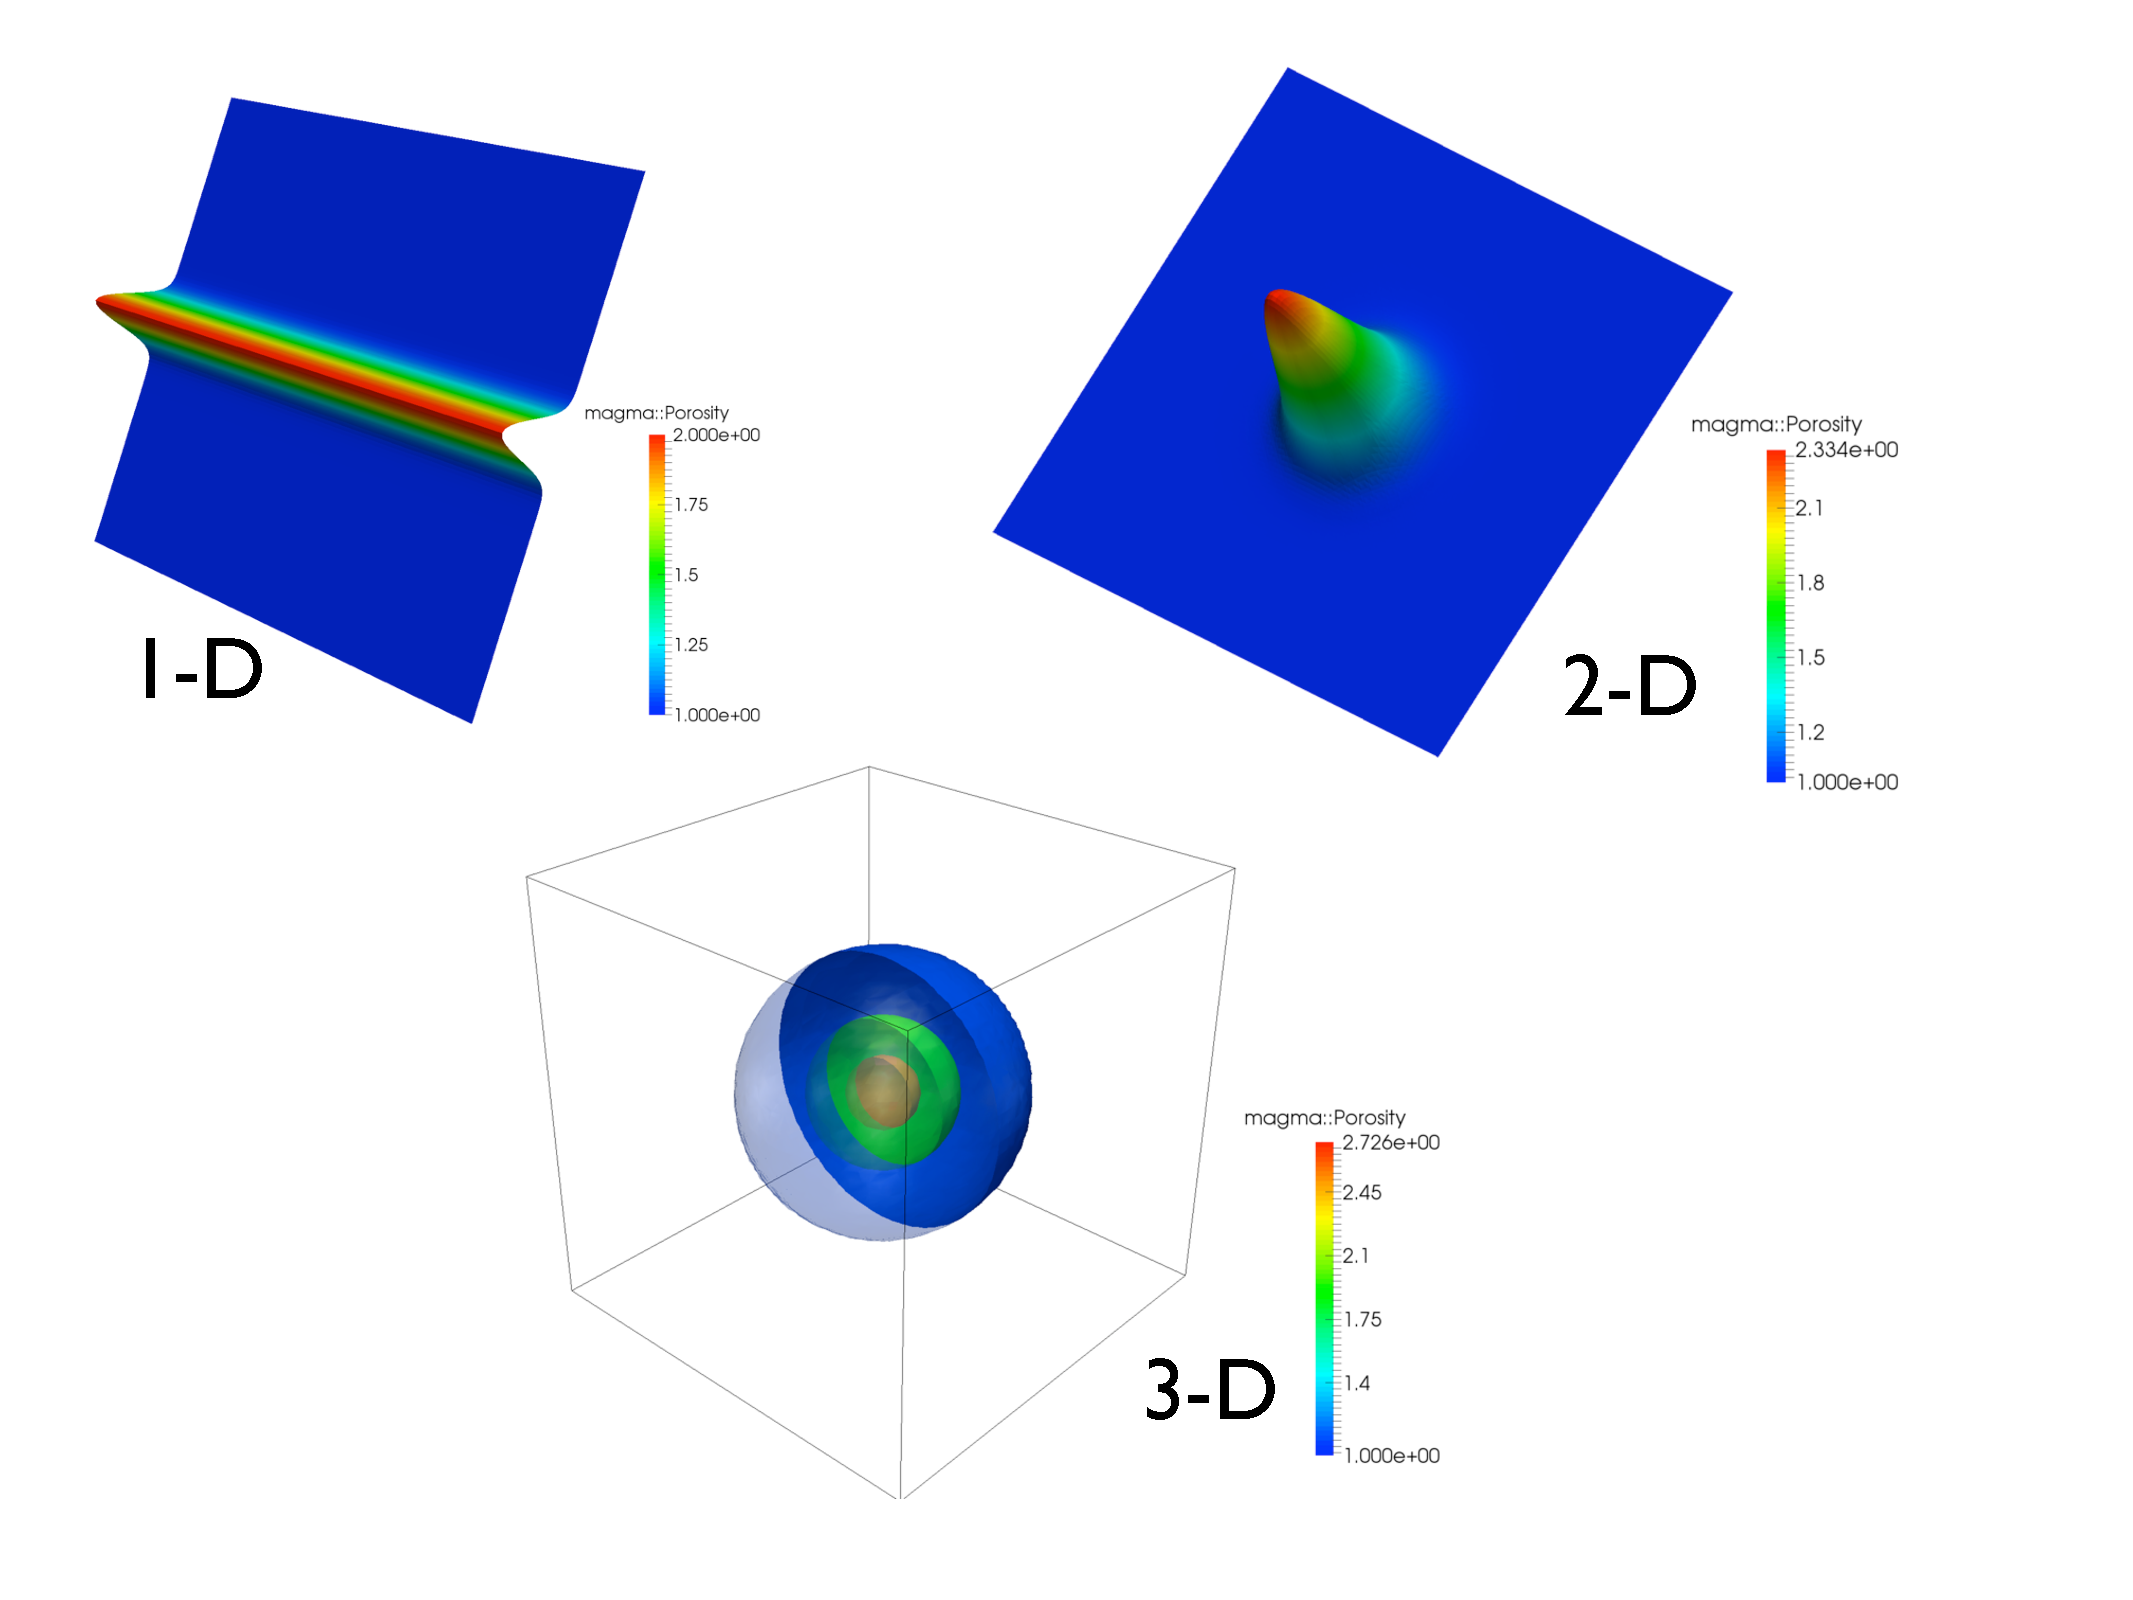
\includegraphics[width=.8\textwidth]{figures/CompositeSolitaryWaves.pdf} 
  \caption{example 1,2 and 3-D magmatic solitary waves that all move
    at speed $c=5$ times the background porosity.}
  \label{fig:SolitaryWavesAllD}
\end{figure}

In the limit of small porosity, the dimensionless governing equations for evolution
of porosity $\phi$ and ``compaction pressure'' $\pcmp$ in a frame
moving at a constant velocity $\Vs$ can be written
\begin{gather}
  \ppt{\phi} + \Vs\cdot\grad\phi = 
  \left(
    \frac{h}{\delta}
  \right)^{2}\frac{\pcmp}{\zeta}  \label{eq:5.1}\\
-\div K \grad\pcmp + \left(
    \frac{h}{\delta}
  \right)^{2}\frac{\pcmp}{\zeta} = \div K \ghat    \label{eq:5.2}
\end{gather}
where $K=\phi^{n}$ is the permeability, $\zeta = 1/\phi^{m}$ is the
bulk viscosity, $\ghat$ is the unit vector in the direction of
gravity.  These equations are scaled by an arbitrary length scale $h$
(usually the system height), in which case  $(h/\delta)$ is  the
system height  in compaction lengths
\begin{gather}
  \delta = \sqrt{\frac{K_{0}\zeta_0}{\mu}}
\end{gather}
Where $K_{0}$ and $\zeta_{0}$ are the permeability and bulk viscosity
at some reference porosity $\phi_{0}\sim0.1-1$\%.  
The compaction length is the intrinsic length scale over which
pressure variations due to obstructions in melt flux propagate as
viscous stresses in the matrix. (See
\cite{spiegelman_flow_1993,spiegelman_flow_1993-1} for more
details). In the limit that the compaction length is much bigger than $h$,
these equations reduce to Darcy flow in a rigid, but translating medium.

Equations (\ref{eq:5.1})--(\ref{eq:5.2}) form a coupled
hyperbolic/elliptic set of equations for the evolution of porosity and
pressure.  For an arbitrary initial condition, these equations will
break up into a series of localized solitary waves that propagate at a
constant speed that depends on amplitude and maintain constant shape
in the absence of collisions or mass transfer between solid and
liquid.  Remarkably, however, we can seek solitary wave solutions in
all dimensions $d$ of the form
\begin{equation}
  \label{eq:5.4}
  \phi(\vec{x},t) = f(r) = f
  \left(
    \sqrt{\sum_{j}^{d-1} x_{j}^{2} + (x_{d} -ct)^{2}}
  \right)
\end{equation}
where $r$ is the radial distance from the peak of the wave.
Substituting $f(r)$ into Equations (\ref{eq:5.1})--(\ref{eq:5.2})
transforms them into a 3rd order, non-linear ODE in $r$.  Except for
some special cases,  these ODE's do not have analytic closed form
solutions, however,  Simpson and Spiegelman
\cite{simpson_solitary_2011}, provides an elegant spectrally accurate
method for numerically calculating solitary wave profiles for all
values of $c,n,m,d$ using the ``sinc collocation method''.  Moreover,
Gideon Simpson has encoded this method in a set of python routines
\texttt{magmasinc} which have been included in this tutorial along
with a set of classes for managing and evaluating the solitary wave
profiles.  For example, the script
\texttt{\$TF\_HOME/share/terraferma/tutorials/porositywaves/python/scripts/see\_wave\_profiles.py} initializes 3 different
solitary waves for $c=5$, $n=3$, $m=1$ and $d=[1,2,3]$, using 150
collocation points.  Figure (\ref{fig:SolitaryWaveProfiles}) shows radial profiles $f(r)$ for these
3 waves.  

\begin{figure}[htbp!]
  \centering
  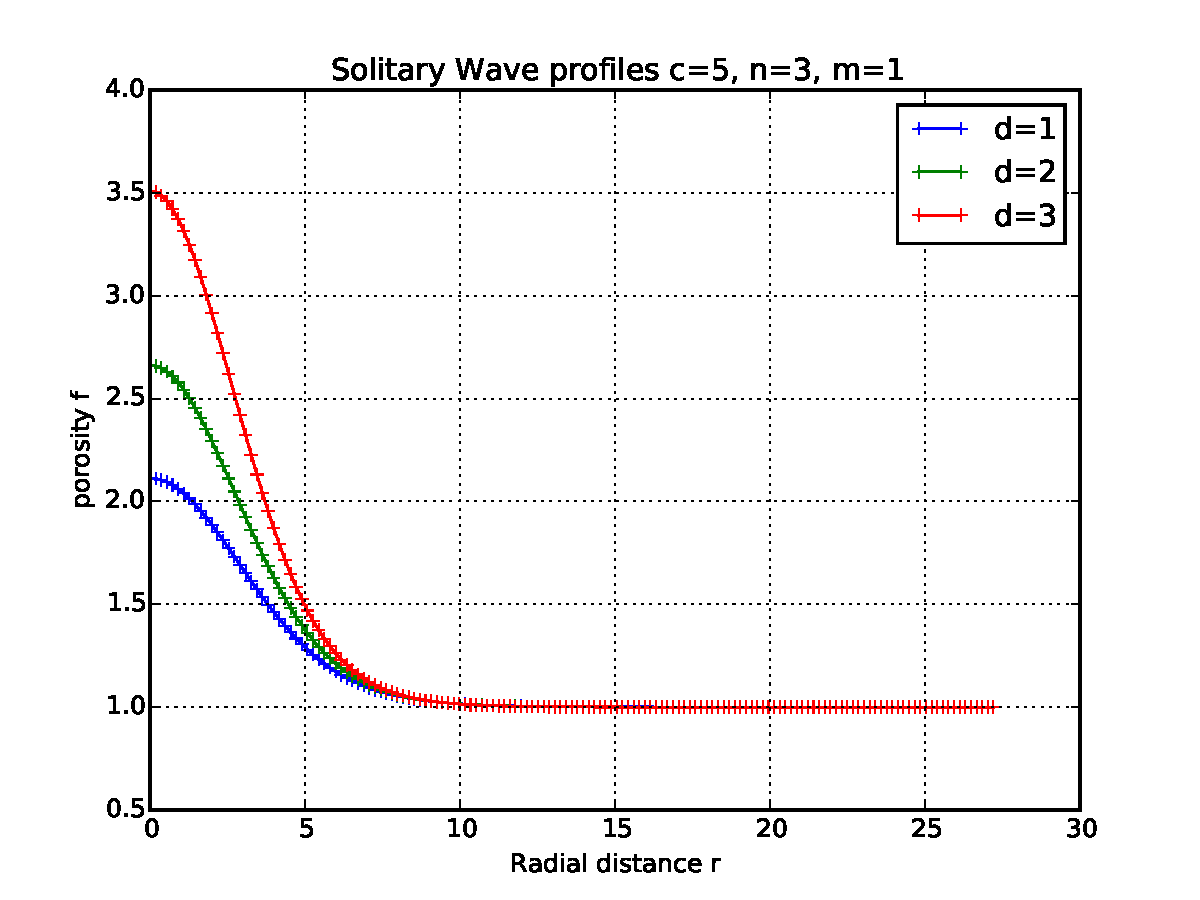
\includegraphics[width=.75\textwidth]{figures/SolitaryWavesProfiles.pdf}
  \caption{Solitary wave profiles $f(r)$ for 1,2 and 3-D waves
    calculated using the pysolwave python package that installs with
    \TF.  All waves travel at speed $c=5$ and have permeability
    exponent $n=3$ and bulk viscosity exponent $m=1$.  Crosses on the
    profiles show the collocation points. All distances in pysolwave
    are scaled to the compaction length in the small porosity
    background ($f=1$).  I.e. these wave profiles extend about 25
    compaction lengths from the wave peak.}
\label{fig:SolitaryWaveProfiles}
 \end{figure}

\subsection{Benchmark problem}
\label{sec:benchmark-problem}

These solitary waves provide an excellent benchmark problem for
testing any model of multi-phase flow.  If chosen as an initial
condition in a frame moving at speed $\Vs = c\ghat$ they should
simply stay put and not change shape.  Any error in position or shape
is strictly due to numerical errors.  As a first problem we will
explore the solitary wave benchmarks as laid out in Simpson and
Spiegelman, 2011 \cite{simpson_solitary_2011} which have the initial
condition of  a single 2-D
or 3-D wave with its peak at the center of a unit square or cube.
$\Vs$ is set to exactly counter the wave propagation.  Boundary
conditions on porosity and pressure are shown in Figure (\ref{fig:solitarywavebcs}). 

\begin{figure}[htbp!]
  \centering
  \def\svgwidth{.8\textwidth}
  \input{figures/solitaryWaveBCs.pdf_tex}
  \caption{Boundary and initial conditions for the solitary wave
    benchmark problem (Simpson and
    Spiegelman,\cite{simpson_solitary_2011}). Porosity and the
    separation flux normal to the top boundary are fixed at the top of
    the domain to provide  a constant input flux of 1.
  Sides are reflection and the bottom boundary condition is ``free
  flux'' which assumes that the gradient of the compaction pressure is
zero such that there is no viscous resistance to volume change on the
bottom boundary. Note, the pressure boundary conditions are all of
Neumann type,  however, unlike Poisson,  Eq.\ (\ref{eq:5.2}) is a
modified Helmholtz problem and is well-posed with all Neumann
conditions (i.e. is not singular)}
  \label{fig:solitarywavebcs}
\end{figure}


\subsection{Variational forms and Discontinuous Galerkin Porosity}
\label{sec:variational-forms}

To write out weak forms for Equations (\ref{eq:5.1}) and
(\ref{eq:5.2}) require choosing stable element pairs for porosity and
compaction pressure.  As Eq.\ (\ref{eq:5.2}) is an elliptic equation
in compaction pressure, standard continuous Galerkin elements (e.g. \Pone
or \Ptwo) have been shown to be adequate for pressure.  Moreover, In the
absence of the $\Vs\cdot\grad\phi$ term, Eq.\ (\ref{eq:5.1}) is
actually an ODE for porosity and continuous elements are also valid.
However, when the $\Vs\cdot\grad\phi$ is included, Eq.\ (\ref{eq:5.1})
becomes a hyperbolic equation for the evolution of porosity in a frame
moving with the solid which can present significant challenges for
accurate solution using continuous Galerkin finite elements.  This term, which
represents advection of porosity by the solid phase is actually
expected for most magma dynamics problems where there is a non-trivial
background flow of solid, such as at a mid-ocean ridge or subduction
zones, and we use it here in the benchmark problem to ``freeze'' the
solitary wave in the box by having the background flow exactly balance
the wave speed $c$.  After some trial and error, we found that using
discontinuous Galerkin elements for porosity works well\footnote{An
  alternative approach is to use Semi-Lagrangian methods which do not
  expressly include the $\Vs\cdot\grad\phi$ term and can be
  implemented in \TF{}.  However, the semi-Lagrangian capability is
  not parallel and we have found, in the end that DG is superior for
  these problems.}.  Here we
will use the mixed discrete function space $\fspace=(\Ptwo,\Ptwodg)$
where $\vec{u}\in\fspace=(p,f)$ (where $p$ will be our  \texttt{ufl}
symbol for pressure, $\pcmp$, and $f$ for porosity $\phi$).

As with the energy equation in thermal convection, we will first
discretize the time derivative in the porosity equation using finite
differences and integrate using a $\theta$ scheme (but we will simply
choose $\theta=1/2$, i.e. a second-order in time trapezoidal integration rule).  
Multiplying by appropriate test functions and integrating by parts, the
variational form of the non-linear problem can be written
\begin{quote}
  \fbox{\parbox{.9\textwidth}{Find $\vec{u}\in \fspace$ such that
      \begin{equation}
         F(\vec{u};\vec{u}_{t}) =0 
      \end{equation}
  for all test functions $\vec{u}_{t}=(p_{t},f_{t}) \in\fspace$.}}
\end{quote}
 where $F(\vec{u};\vec{u}_{t}) = F_{p} + F_{f}$ with
\begin{align}
         F_{p} =  & \int_\Omega \left(
\grad p_{t}\cdot K_{i}
                    \left[
                    \grad p_{i} + \ghat
                    \right] 
+ \chi_{i}p_{t}p_{i}
 \right])d\vec{x}  - \int_{\partial\Omega} p_{t}
                    \left[
                    K_{i}(\grad p_{i} + \ghat)\cdot\vec{n}
                    \right] ds\\
 F_{f} =& \int_\Omega f_{t}[ f_{i} -f_{n}
          -\frac{dt}{2}(\chi_{n}p_{n}+\chi_{i}p_{i})]d\vec{x}
          \nonumber\\
          & -\int_{\Omega} 
            dt\left(
            f_{1/2}\Vs\cdot\grad f_{t}
            +f_{t}f_{1/2}\div\Vs
            \right)d\vec{x}\nonumber\\
          & + \int_{\partial\Omega}dt f_{t}f_{1/2}\Vs\cdot\vec{n} ds
            \nonumber\\
          & + \int_{\mathrm{internal\,  facets}} dt [[f_{t}]]f_{1/2}^{*}\Vs\cdot\vec{n}dS\label{eq:5.5}\\
\nonumber \\
  F = & F_{p} + F_{f} \label{eq:5.systemresidual}
\end{align}
where 
\begin{align*}
  f_{1/2} = & \frac{1}{2}(f_{n} + f_{i})\\
  \chi_n = & 
             \left(
             \frac{h}{\delta}
             \right)^{2}f_{n}^{m}\\
\chi_i = & 
             \left(
             \frac{h}{\delta}
             \right)^{2}f_{i}^{m}\\
K_{i}    = & f_{i}^{n}\\
\end{align*}
are the interpolated porosity at the half-time step, bulk viscosity
terms at the old and new times and permeability at the new time. In
addition
\begin{align*}
  [[f_{t}]] = f_{t}^{+} - f_{t}^{-}
\end{align*}
is the ``jump operator'' which 
measures the difference in a function across a facet (the $^{+}$ and
$^{-}$ denote the one sided limits of the function on either side of
the facet).  For continuous elements the jump operator is zero.

These variational forms appear somewhat more complicated than those of
our previous examples for several reasons\footnote{not counting the fact, that
most people are not familiar with these equations}.  First,  the
Neumann flux boundary conditions add additional surface integrals to
the forms.  But more significantly the discontinuous Galerkin elements
for porosity add additional complexity to the variational forms for
the porosity residual.  The last three lines of Eq.\ (\ref{eq:5.5}) all arise from
integration by parts of the advective term over each element
\begin{displaymath}
  \int_{\Omega} f_{t}\Vs\cdot\grad f_{1/2} d\vec{x} = \sum_e \int_{\Omega_{e}} f_{t}\Vs\cdot\grad f_{1/2} d\vec{x}
\end{displaymath}
which generates body integrals over the domain,  surface integrals
over the external boundaries of the domain,  and because of the
discontinuous nature of the basis functions,  integrals over the
internal facets between cells.  This last term, as written, is
actually ambiguous as the porosity
$f_{1/2}$ is  multi-valued along the facets (thus the $*$ notation),
however, we still need to specify a continuous normal flux across each
facet 
\begin{equation}
  \label{eq5:flux}
    q = f_{1/2}^{*}\vec{V}\cdot\vec{n}
\end{equation}
Since, for this problem, $\vec{V}$ is already continuous, the choice
comes down to choosing an appropriate value of the porosity at the
facet. While there are many choices for this (and many are numerically
unstable), here we  will use an upwind scheme to select the
porosity from the cell that is being advected from.  Note, this is
somewhat different from a finite volume upwind scheme that uses the
cell average of the donor cell which can lead to significant numerical
diffusion.  For these problems, where the porosity is essentially smooth,
this upwind scheme is quite accurate, but avoids the spurious
oscillations produced using continuous elements.

The weak form of the residual in UFL looks reasonably
similar, however, there are some additional notation required for
describing discontinuous elements.  For this problem we will actually
split the UFL into two parts.  The first is a global declaration of
some useful UFL symbols that can be used in all forms
\begin{lstlisting}[style=UFL]
# Global parameters for porosity pressure residual 
#
# permeability
K = f_i**n

#inverse bulk viscosity function
Xi_i = h_squared*f_i**m
Xi_n = h_squared*f_n**m

#porosity at a half-time step
f_half = 0.5*(f_i + f_n)

# domains for assembly of surface integrals
ds_top   = ds(4)
ds_bottom = ds(3)
ds_left  = ds(1)
ds_right = ds(2)
\end{lstlisting}
The last four lines describe some convenience symbols for the
surface integrals on the external boundaries. 

The actual UFL for the residual $F$ is then
\begin{lstlisting}[style=UFL]
#facet normal on pressure
pn = FacetNormal(p.cell())

# body integral for pressure
bp = inner(grad(p_t), K*(grad(p_i) + ghat)) + p_t*p_i*Xi_i 

# surface integral terms for fluid flux 
sptop   = -p_t*inner(ghat, pn) # force -K[grad(p) + ghat].n = 1 on top boundary
spbot   = -p_t*inner(K*ghat, pn) #"free flux BC where inner(grad(p),pn)=0

#pressure residual
Fp = bp*dx + sptop*ds_top + spbot*ds_bottom

#outward facing facet normal for porosity cell
fn = FacetNormal(f.cell())
# facet normal solid velocity
vn = dot(W, fn)
# rectified normal solid velocity ( = vn if outflow, 0 if inflow)
vnout = 0.5*(vn + abs(vn))

# body integrals for porosity
bfm = f_t*(f_i - f_n - dt*0.5*(p_i*Xi_i + p_n*Xi_n))
# body integrals for advective integrals
bfa = - dt*dot(grad(f_t), W*f_half) - dt*f_t*div(W)*f_half

# all porosity body integrals
bf = bfm + bfa

#surface integrals - external boundaries
sftop = dt*f_t*vn  # set phi=1 on the top
sfbot = dt*f_t*(vn*f_half)
sfside = dt*f_t*(vnout*f_half)  # outflows but 0 if inflow

# surface integrals over interior facets
upwindfacetflux = vnout('+')*f_half('+') - vnout('-')*f_half('-')
sffacet = dt*jump(f_t)*upwindfacetflux

# porosity residual
Ff =  bf*dx + sftop*ds_top + sfbot*ds_bottom + sfside*ds_left + sfside*ds_right + sffacet*dS

# total residual
F = Fp + Ff
\end{lstlisting}

\pagebreak{}
The key line in the above ufl are \#16--19 and  \#35
\begin{lstlisting}[style=UFL]
# facet normal solid velocity
vn = dot(W, fn)
# rectified normal solid velocity ( = vn if outflow, 0 if inflow)
vnout = 0.5*(vn + abs(vn))
...
upwindfacetflux = vnout('+')*f_half('+') - vnout('-')*f_half('-')
\end{lstlisting}
which sets the flux $q$ Eq.\ (\ref{eq5:flux}) to be the value of the
porosity from the side of the facet that is an outflow.  Note that
\texttt{vnout} evaluates to zero for an inflow facet and \texttt{vn}
the normal component of the velocity for an outgoing facet (and
\texttt{vn}$\geq 0$).

\section{Solution using \TF}
\label{sec:solution-using-tf}

While the details of the solitary wave benchmarks appear significantly
different from that of thermal convection (Chapter
\ref{cha:thermal-convection}), the structure of the problem is quite
similar and reasonably straightforward to set up in \TF{}.  We could
start with an old \texttt{.tfml} file from thermal convection but it
probably makes more sense to begin with a blank \texttt{.tfml} file
and fill it in sequentially.  Where features, such as an adaptive time
stepper, can be reused from the thermal convection problem, we will
use the (extremely useful) cut and paste functions in diamond to reuse
option blocks from other models.

A fully worked out \texttt{tfml} file for the benchmark problem 
can be found in
\texttt{\$TF\_HOME/share/terraferma/tutorials/porositywaves/benchmark/magmawaves.tfml},
along with an accompanying testharness file \texttt{magmawaves.shml}
for testing.  A typical solution is shown in Figure \ref{fig:solitarywavebcs}.

To build this model in \TF{} from scratch, do the following
\begin{steps}{Step}
  \item Make a new tfml file
  \begin{lstlisting}[style=Bash]
$ mkdir mybenchmark
$ chdir mybenchmark
$ diamond magmawaves.tfml &
  \end{lstlisting}%$
\item \textbf{Set the geometry:} Here we will use a 2-D UnitSquare mesh.
  \begin{steps}{step}
  \item Set dimension to 2 (this can only be done once)
  \item Choose \texttt{mesh (Mesh)} 
  \item Choose \texttt{source (UnitSquare)}
  \item Set \texttt{number\_cells} to $32\times32$
  \item Set \texttt{diagonal} to \texttt{right/left}
  \end{steps}
\item \textbf{Set io parameters}
  \begin{steps}{step}
  \item Set \texttt{output\_base\_name} to \texttt{magmawaves}
  \item Set \texttt{visualization->element} to (P2DG)
  \item Set dump-periods for visualization and statistics
    output.  Under \texttt{dump\_periods} 
    \begin{itemize}
    \item Activate \texttt{visualization\_period} and set to
      0.05
    \item Activate \texttt{statistics\_period} and set to
      0.025
  \end{itemize}
\item Activate \texttt{checkpointing} and set
  \texttt{checkpointing\_period} to 0.05.  We will need checkpoint
  files at every visualization time to be able to test the accuracy of
  the solution using an external python package.
  \end{steps}
\item \textbf{Set Time Stepping parameters}
  \begin{steps}{step}
  \item Activate \texttt{timestepping}
  \item Set \texttt{current\_time} to 0.0
  \item Set \texttt{finish\_time} to 0.5
  \item Open \texttt{timestep}
  \item Open \texttt{coefficient (Timestep)} and unfold all the way to \texttt{constant}
    \begin{itemize}
    \item Set \texttt{ufl\_symbol (global)} to \texttt{dt}
    \item Set \texttt{value (WholeMesh)->constant } to 0.  We're
      going to use adaptive time-stepping with the initial \texttt{dt=0} trick
      that we used for thermal convection.
    \end{itemize}
  \item Activate \texttt{adaptive} and unfold \texttt{constraint}
    \begin{itemize}
    \item Set \texttt{constraint} name to \texttt{Courant}
      (and don't forget to hit carriage return for these name strings)
    \item Set \texttt{system} name to \texttt{CourantNumber}.  We'll
      add this system later by borrowing pieces from the thermal
      convection models.
    \item Set  \texttt{field} name to \texttt{CourantNumber}
    \item Set \texttt{requested\_maximum\_value} to 0.25 (which is
      appropriated for a $c=5$ wave and we will change this through
      the testharness as well).
    \item Activate \texttt{adapt\_period} and set to 2.0 (this won't actually try
      to re-adapt through the run giving a constant time-step)      
    \end{itemize}
  \end{steps}
\item Unfold \texttt{global\_parameters}. Here we will set some global
  ufl symbols that can be used across all systems along with some
  dolfin specific parameters to allow parallel computation with DG elements.
  \begin{steps}{step}
  \item Activate \texttt{ufl} and in the Data box input
    \begin{lstlisting}[style=UFL]
# Global parameters for porosity pressure residual 

# permeability
K = f_i**n

#inverse bulk viscosity function
Xi_i = h_squared*f_i**m
Xi_n = h_squared*f_n**m

#porosity at a half-time step
f_half = 0.5*(f_i + f_n)

# domains for assembly
ds_top   = ds(4)
ds_bottom = ds(3)
ds_left  = ds(1)
ds_right = ds(2)
    \end{lstlisting}
(which are the same as those listed in Section
\ref{sec:variational-forms}).  Note, any changes to this global ufl
section will force a recompile of the model so use these sparingly and
with some care.  
\item Activate \texttt{dolfin} and unfold
\item Activate \texttt{ghost\_mode} and set to
  \texttt{shared\_facet}.  This will allow proper assembly of facet
  integrals in parallel (this is a dolfin parameter that we
  unfortunately need to pass through).
  \end{steps}
\item Set the \texttt{system} (and actually solve something).
  \begin{steps}{step}
  \item Set the \texttt{system} name to \texttt{magma}
  \item Choose \texttt{mesh (Mesh)} to use the defined mesh
  \item Set the \texttt{ufl\_symbol (global)} to \texttt{us}.  Again,
    this is the \texttt{ufl} symbol for the entire mixed system of
    pressure and porosity.
  \item Activate a \texttt{field}, name it \texttt{Pressure} and unfold
    \begin{itemize}
    \item Set the \texttt{ufl\_symbol (global)} to \texttt{p}
    \item Unfold \texttt{type (Function)} and set the element to
      \texttt{(P2)} (this should automatically be \texttt{rank
        (Scalar)}
    \item Unfold \texttt{initial\_condition (WholeMesh)} and set a
      \texttt{constant} value of 0.0
    \item Unfold \texttt{diagnostics} and activate
      \texttt{include\_in\_visualization} and \texttt{include\_in\_statistics}
    \end{itemize}
\item Activate a second \texttt{field}, name it \texttt{Porosity} and unfold
    \begin{itemize}
    \item Set the \texttt{ufl\_symbol (global)} to \texttt{f}
    \item Unfold \texttt{type (Function)} and set the element to
      \texttt{(P2DG)} (this should automatically be \texttt{rank
        (Scalar)}
    \item Unfold \texttt{initial\_condition (WholeMesh)} and choose
      \texttt{python}.  Now the fun begins. To use the pysolwave
      utilities for easily generating solitary wave profiles,  we have
      written a python class \texttt{tfsolitarywave},  which reads
      parameters from a \texttt{.tfml} file (namely this one) and
      calculates solitary wave profiles.  To invoke it, add the
      following to the data window.
      \begin{lstlisting}[style=Python]
# Initialize to single solitary wave profile 
# using PySolwave routines 
# This header will act as a global header to all subsequent def val instances
# (with great power comes great responsibility)

from pysolwave.tfsolitarywave import TFSolitaryWave
from glob import glob

tfmlfile = glob("magmawaves.tfml")[0]

#initialize solitary wave object from tfmlfile
tfswave = TFSolitaryWave(tfmlfile)

# print out some info about the solitary wave 
print "Solitary Wave information:"
print "c=",tfswave.swave.c, " n =",tfswave.swave.n, " d=",tfswave.swave.d, " r_max=",tfswave.rmax

print "f=",tfswave.swave.f

# python function for setting initial condition
import numpy as np
def val(x):
  global tfswave,np
  f = tfswave.eval(np.array(x))
  return f
\end{lstlisting}
\textbf{CAUTION:} if you copy the text from the pdf into diamond, be
very careful to maintain indentation and be aware that copy/paste may
from this tutorial may introduce non-ascii characters into diamond
which will cause an error (In particular, the double quotes
\texttt{``} need to be edited to simple ascii ones.

The source code for \texttt{tfsolitarywave.py} can be found in
\texttt{\$TF\_HOME/share/terraferma/tutorials/porositywaves/python/pysolwave/tfsolitarywave.py}. In
particular it assumes a number of default parameters and locations to
be present in the \texttt{.tfml} file.  It's full syntax is
\begin{lstlisting}[style=Python]
class TFSolitaryWave:
    """ class for calculating and evaluating solitary wave profiles
        with data from  TerraFERMA .tfml input files
    """

    def __init__(self,tfml_file,
       system_name='magma',p_name='Pressure',f_name='Porosity',
       c_name='c',n_name='n',m_name='m',d_name='d',N_name='N',
       h_squared_name='h_squared',x0_name='x0'):
        
     """read the tfml_file and use libspud to populate the internal parameters

        c: wavespeed
        n: permeability exponent
        m: bulk viscosity exponent
        d: wave dimension
        N: number of collocation points
        x0: coordinate wave peak
        h_squared:  the size of the system in compaction lengths
                          squared (h/delta)**2
        """
\end{lstlisting}
Thus the default is to look for the system named \texttt{magma}, for
fields and coefficients with names \texttt{Pressure},
\texttt{Porosity}, \texttt{c,n,m,d,N,x0} and \texttt{h\_squared}.  Any
changes in these names just need to be passed to
\texttt{TFSolitaryWave}.  Here however, we will just set up a set of
coefficients with the appropriate names.
        \item Set the upper Dirichlet boundary condition $\phi=1$.
    \begin{itemize}
    \item Activate a new boundary condition, name it \texttt{top} and unfold
    \item Set \texttt{boundary\_ids} to 4 (upper boundary)
    \item Set \texttt{sub\_components (All)}$\rightarrow$\texttt{type
        (Dirichlet)}$\rightarrow$\texttt{constant} to 1.
    \end{itemize}
  \item Unfold \texttt{diagnostics} and activate
      \texttt{include\_in\_visualization} and \texttt{include\_in\_statistics}

    \end{itemize}

  \item Activate a lot of coefficients and set their values.  We'll
    start with the physical parameters, then the solitary wave
    parameters needed for \texttt{TFSolitaryWave}
    \begin{itemize}
    \item Set the background advection velocity \texttt{W}.  Activate
      a coefficient named \texttt{W} and unfold and set
      \begin{itemize}
      \item  \texttt{ufl\_symbol (global)} \texttt{W}
      \item \texttt{type (Constant)}
      \item \texttt{rank (Vector)}
      \item \texttt{value (WholeMesh)}
      \item \texttt{constant (dim)} to $[0,-5.]$ (i.e. $-c$ in the $z$ direction).
      \end{itemize}
    \item Set the gravity unit vector $\ghat=[0,-1]$.  Add another
      vector valued coefficient named \texttt{ghat}, with \texttt{ufl\_symbol (global)}
      \texttt{ghat} and constant value = $[0,-1.]$
    \item Set the wavespeed $c=5.$  Activate
      a coefficient named \texttt{c} and unfold and set
      \begin{itemize}
      \item  \texttt{ufl\_symbol (global)} \texttt{c}
      \item \texttt{type (Constant)}
      \item \texttt{rank (Scalar)}
      \item \texttt{value (WholeMesh)}
      \item \texttt{constant} = 5.
      \end{itemize}
    \item Repeat for the rest of the scalar wave parameters
      \begin{itemize}
      \item \texttt{n}=3
      \item \texttt{m}=0
      \item \texttt{d}=2
      \item \texttt{N}=150
      \item \texttt{h\_squared}=4096 ($(h/\delta)=64$)
      \end{itemize}
    \item And set a vector valued Constant coefficient \texttt{x0} for
      the location of the wave peak to $[0.5,0.5]$

    \end{itemize}
  \item Name the \texttt{nonlinear\_solver} \texttt{Solver} and unfold
    \begin{itemize}
    \item Set the Residual \texttt{F}.  \emph{Carefully} copy the ufl for the
      residual $F$ described
      above in \texttt{form (Residual)} and set the
      \texttt{ufl\_symbol (solver)} to \texttt{F}.  In particular, if
      you copy and paste from this pdf manual, you will introduce some
      non ascii characters into the ufl (in this case the \texttt{'}
      single quote character,  \texttt{'}).  This will need to be
      replaced in the ufl in diamond.
    \item Set the Jacobian \texttt{J}.  Copy the \texttt{ufl}
      \begin{lstlisting}[style=UFL]
        J = derivative(F, us_i, us_a)
      \end{lstlisting}
      to \texttt{form (Jacobian)} and set the \texttt{ufl\_symbol
        (solver)} to \texttt{J}
    \item Set \texttt{relative\_error} to \texttt{1.e-7}
    \item Activate \texttt{absolute\_error} and set to \texttt{1.e-11}
    \item Set \texttt{max\_iterations} to \texttt{50} (it shouldn't
      take that many)
    \item Activate \texttt{monitors}$\rightarrow$\texttt{residual} to
      log the non-linear residuals.
    \end{itemize}
  \item Set the Linear solver
    \begin{itemize}
    \item Choose \texttt{iterative\_method (fgmres)} (flexible
      gmres). Unfold and set
      \begin{itemize}
      \item \texttt{restart} $=$ 30
      \item \texttt{relative\_error} $=$ \texttt{1.e-7}
      \item \texttt{absolute\_error} $=$  \texttt{1.e-12}
      \item \texttt{max\_iterations} $=$  \texttt{20}
      \item and activate \texttt{monitors}$\rightarrow$\texttt{preconditioned\_residual}
      \end{itemize}

    \item Choose \texttt{preconditioner (fieldsplit)} and unfold
      \begin{itemize}
      \item Name the first \texttt{fieldsplit} \texttt{Pressure}.
        Here we will just apply the hypre preconditioner to the
        pressure field.
        \begin{itemize}
        \item Activate \texttt{field} and name it
          Pressure.
        \item Unfold the \texttt{linear\_solver}
        \item Choose \texttt{iterative\_method (preonly)} 
        \item Choose \texttt{preconditioner (hypre)} 
        \end{itemize}
      \item Activate a second \texttt{fieldsplit} and name it
        \texttt{Porosity}.  Here we will apply an eisenstat
        preconditioned gmres iterative solver which we have found
        works quite well for these problems. (the Option Properties
        Description in diamond, provides a brief discussion of the eisenstat preconditioner).
        \begin{itemize}
        \item Activate \texttt{field} and name it
          Porosity.
        \item Unfold the \texttt{linear\_solver}
        \item Choose \texttt{iterative\_method (gmres)}, unfold and set
         \texttt{restart}$=$30, \texttt{relative\_error}$=$1.e-7, \texttt{max\_iterations}$=$50
        \item Choose \texttt{preconditioner (eisenstat)} 
        \end{itemize}
      \end{itemize}
    \end{itemize}
    
  \item If you want, add some functionals to calculate the integral of the
    pressure and porosity.
    \begin{itemize}
    \item Activate a functional and name it \texttt{PressureIntegral}
      and unfold.
    \item set the ufl for the functional to
      \begin{lstlisting}[style=ufl]
        int = p*dx
      \end{lstlisting}
    \item set the \texttt{ufl\_symbol (functional)} to \texttt{int}
    \end{itemize}
  \item Add a functional to calculate the integral of the porosity
    which should be constant over time. Here we can use the cut and
    paste feature of diamond.  Click on \texttt{functional
      (PressureIntegral)} to highlight that tab.  Using the edit menu
    in diamond, choose copy,  then highlight a new functional tab and
    using the edit menu choose paste.\footnote{There are also some
      mouse shortcuts for cutting and pasting but these will vary by
      operating system}  This will duplicate the
    pressure functional.  Now simply change the name from
    \texttt{PressureIntegral} to \texttt{PorosityIntegral} and the ufl to
    \begin{lstlisting}[style=ufl]
        int = f*dx
     \end{lstlisting}
  \end{steps}
\item The final step is to add a system to calculate the Courant
  number for the adaptive time-stepper.  Again,  here we can use the
  copy and paste features of diamond to reuse the CourantNumber system
  we already developed for Thermal Convection
  \begin{steps}{step}  
  \item Using diamond, open the \texttt{tfml} file for
    thermal convection
    \texttt{\$TF\_HOME/share/terraferma/tutorials/thermalconvection/isoviscous/
      newton\_direct/convection.tfml}
  \item Highlight \texttt{system (CourantNumber)} and use
    \texttt{Edit}$\rightarrow$\texttt{Copy} to copy the entire system
    to the clipboard.
  \item move to your \texttt{magmawaves.tfml} window, highlight the
    unactivated system at the bottom and use
    \texttt{Edit}$\rightarrow$\texttt{Paste} to insert the full
    Courant number system. \textbf{Caution:} when cutting and pasting
    between models (and even within a model, there is always the
    chance of duplicating \texttt{ufl\_symbols} or introducing
    inconsistencies so each option should be checked. In this case
    there will be a few things to patch up.
  \item Unfold \texttt{system (CourantNumber)} and note that the
    \texttt{ufl\_symbol (global)} for the field \texttt{CourantNumber}
    is set to \texttt{c}, which we have already used for wavespeed.
    We will change the name here to \texttt{cfl} and then make
    subsequent changes to the Residual \texttt{ufl}.
  \item Unfold the \texttt{nonlinear\_solver (Solver)} and expose the
    \texttt{residual} which should look like
    \begin{lstlisting}[style=UFL]
# Finite volume style estimate of Courant number
# calculate the outward facing normal component of velocity for each facet
n = FacetNormal(c_e.cell())
vn = dot(v_i, n)
vout = 0.5*(vn + abs(vn))

# project the cell integral of the outgoing flux from each cell
F = c_t*c_i*dx - c_t('+')*vout('+')*dt('+')*dS - c_t('-')*vout('-')*dt('-')*dS - 
c_t*vout*dt*ds(1) - c_t*vout*dt*ds(2) - c_t*vout*dt*ds(3) - c_t*vout*dt*ds(4)
    \end{lstlisting}
and modify all occurrences of \texttt{c} to \texttt{cfl} and change
\texttt{v\_i} to \texttt{W\_i} to record the proper solid velocity
field.  Your final ufl should look like
\pagebreak{}
\begin{lstlisting}[style=UFL]
# Finite volume style estimate of Courant number
# calculate the outward facing normal component of velocity for each facet
n = FacetNormal(cfl_e.cell())
vn = dot(W_i, n)
vout = 0.5*(vn + abs(vn))

# project the cell integral of the outgoing flux from each cell
F = cfl_t*cfl_i*dx - cfl_t('+')*vout('+')*dt('+')*dS - cfl_t('-')*vout('-')*dt('-')*dS -
cfl_t*vout*dt*ds(1) - cfl_t*vout*dt*ds(2) - cfl_t*vout*dt*ds(3) - cfl_t*vout*dt*ds(4)
\end{lstlisting}


  \end{steps}



\end{steps}

That should conclude construction of the basic model \texttt{.tfml}
file.  To build it use
\begin{lstlisting}[style=Bash]
$ tfbuild magmawaves.tfml -a magmawaves.tfml
$ cd build
$ make
$ make run 
\end{lstlisting}
The extra \texttt{-a} argument adds a copy of magmawaves.tfml to the
build directory which will be necessary for \texttt{TFSolitaryWave} to
work.  If everything is working you should generate a set of images of a
stationary solitary wave.  To go further, you should look at the
testharness file \texttt{magmawaves.shml} in the tutorials directory
that runs this problem over a range of mesh resolutions and time-steps
and reinvokes \texttt{TFSolitaryWave} to calculate velocity and phase
errors against the exact solutions and produces an output .tex table
as well as checks the integrals of porosity and pressure.
\begin{table}[h]
  \centering
  \caption{output table showing relative phase and velocity errors for the
    solitary wave benchmark}
  \label{benchmark_table}
\begin{tabular}{c|cccc}
\hline
 $N$ & $h_{cell}/\delta$ & $c\Delta t/\delta$ & $||e||_2/||\phi_c||_2$ &$\Delta c/c$\\
\hline
 16 & 4 & 0.25 & 2.08864e-03 & 1.23076e-03 \\
 16 & 4 & 0.50 & 2.08864e-03 & 1.23065e-03 \\
 16 & 4 & 1.00 & 2.08862e-03 & 1.23158e-03 \\
 32 & 2 & 0.25 & 2.09965e-04 & -2.03282e-05 \\
 32 & 2 & 0.50 & 2.09965e-04 & -2.03311e-05 \\
 32 & 2 & 1.00 & 2.09973e-04 & -2.04066e-05 \\
 64 & 1 & 0.25 & 2.52327e-05 & -3.27680e-06 \\
 64 & 1 & 0.50 & 2.52327e-05 & -3.27684e-06 \\
 64 & 1 & 1.00 & 2.52328e-05 & -3.27943e-06 \\
\hline
\end{tabular}
  
\end{table}


%\pagebreak{}
\section{Themes and Variations}
\label{sec:themes-variations}

The single solitary wave benchmarks are extremely important for
verifying the accuracy of numerical schemes for magma migration as
they are fully non-linear solutions with well understood behavior that
rapidly expose any numerical artifacts with a given scheme.  That
said,  they're still a bit dull as if they are working well,  the
result is a single static solitary wave that doesn't do anything.
However with a few small changes to the tfml files  there are a few
more interesting things that can be explored with the solitary waves. 

\begin{figure}[htbp!]
  \centering
  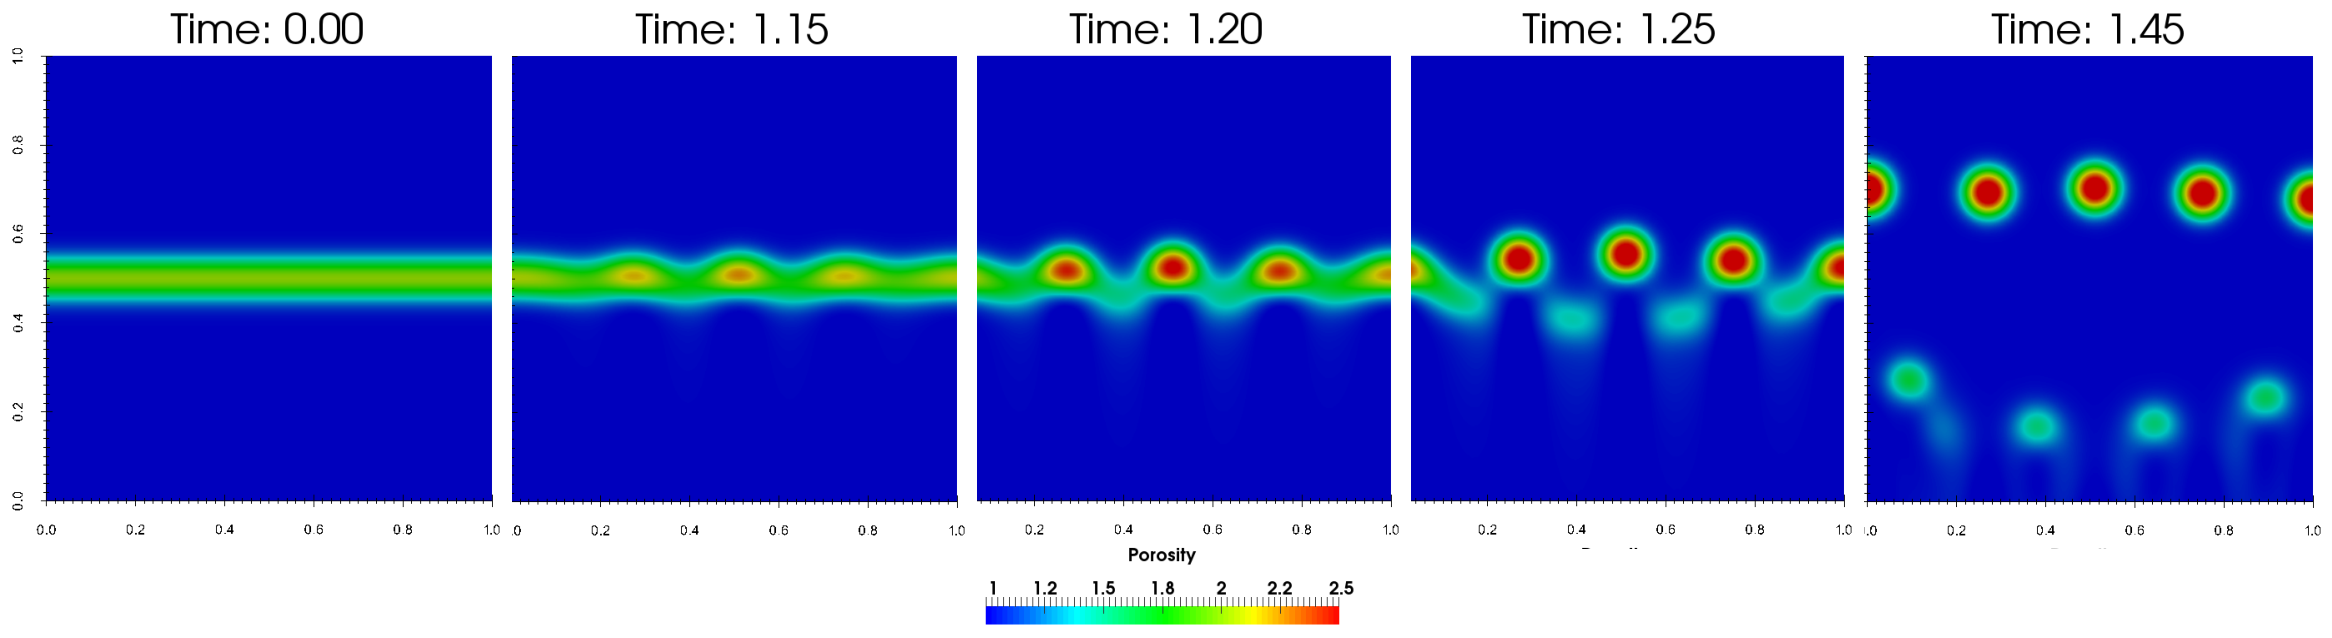
\includegraphics[width=\textwidth]{figures/1dto2d.pdf}
  \caption{Instability of a 1-D solitary wave ($c=5$, $n=3$, $m=0$,
    $d=1$) in 2 dimensions. This calculation is done in a frame moving
    with the initial solitary wave $W=-5$, such that the wave appears
    to be stationary. The initial 1-D wave propagates for some time
    ($t\approx 1$) before developing local melt concentrations that
    rapidly form into stable 2-D solitary waves (e.g. $t=1.15-1.25$)
    plus some smaller waves and background radiation.  The large 2-D
    waves, when well separated, propagate with constant shape and speed.}
  \label{fig:1dto2d}
\end{figure}

\subsection{Stability of solitary waves}
\label{sec:stab-solit}


It has long been known that in each embedding dimension (1, 2 or 3-D)
there are stable solitary wave solutions, however, lower dimensional
waves are always unstable to higher dimensional waves
\cite{scott_magma_1986,barcilon_nonlinear-waves_1986,barcilon_solitary_1989}.
For example, Figure \ref{fig:1dto2d} demonstrates the instability of a
1-D solitary wave in 2-D dimensions with the eventual break down of the
1-D wave into a set of 2-D solitary waves plus background radiation.
A fully worked out example for this problem can be found in
\texttt{\$TF\_HOME/share/terraferma/tutorials/porositywaves/1dto2d/magmawaves.tfml}
along with a testharness file.  These models take some time to run so
the included testharness file runs this problem in parallel on two
processors.  If you have more or less cores, it is easy to change this
by adjusting the \texttt{number\_processes} tab in
\texttt{magmawaves.shml}.

The principal changes to the \texttt{tfml} file from the benchmark
problem, are
\begin{itemize}
\item change the value of the wave dimension \texttt{d} from 2 to 1
\item increase the \texttt{finish\_time} to about 1.5 (see below)
\item modify the adaptive time-stepper to try and keep up with the
evolving solution.  In the example we
have used a Courant number adaptive time-step however instead of
using the solid velocity, we adapt to the melt-separation velocity.
\begin{equation}
  \label{eq:sep-velocity}
\vec{q} =\vf - \Vs  = -\frac{K}{\phi}
\left[
  \grad\pcmp + \ghat
\right] 
\end{equation}
\item To do this we will need another system \texttt{SeparationVelocity}
  \begin{itemize}
  \item Create a new system called \texttt{SeparationVelocity} that
    calculates the separation velocity as a projection onto $[P_{1},P_{1}]$ using the ufl
\begin{lstlisting}[style=UFL]
F = inner(q_t,(q_i + K/f_i*(grad(p) + ghat)))*dx
\end{lstlisting}
\item For efficiency use a simple (SOR,CG) linear solver for the
  projection. (see the example file)
  \end{itemize}
\item Change the velocity in the system \texttt{CourantNumber} from
  the solid velocity \texttt{W\_i} to \texttt{q\_i}. This approach has the advantage of
taking a smaller time step as the waves grow, because larger waves
have larger separation velocities.  
\item Most importantly,  we add an additional
  \texttt{nonlinear\_solver}  \texttt{InitialGuess} to the system
  \texttt{magma}.  This solver simply takes a first order Euler step
  to update the porosity using the pressure at the previous time-step
  (the pressure is just formulated as a projection problem but not
  solved for).  By starting with a guess for the evolved porosity,
  this extra solve greatly increases the rate of convergence and
  overall robustness and performance of this model. To add this solver
  \emph{before} the main Newton solver (\texttt{Solver})
  \begin{itemize}
  \item Copy the \texttt{nonlinear\_solver} tab \texttt{Solver} and
    paste it over the greyed out \texttt{nonlinear\_solver} tab below
    it.
  \item Rename the first solver \texttt{InitialGuess}
  \item Edit the UFL for the residual so that the pressure residual is
    just a projection problem, i.e.
    \begin{lstlisting}[style=UFL]
#pressure residual (just project)
Fp = p_t*(p_i - p_n)*dx
    \end{lstlisting}
  \item And change the porosity residual so that it takes an Euler
    step (i.e. only depends on \texttt{p\_n} not \texttt{p\_i}
    i.e. change one line to
    \begin{lstlisting}[style=UFL]
# body integrals for porosity
bfm = f_t*(f_i - f_n - dt*p_n*Xi_n)
    \end{lstlisting}
  \item To just solve for porosity in the initial guess, change the
    fieldsplit preconditioner to
    \begin{itemize}
    \item \texttt{composite\_type} = additive
    \item under \texttt{fieldsplit (Pressure)} set the
      \texttt{iterative\_method} to \texttt{preonly} and the
      \texttt{preconditioner} to none
    \end{itemize}



  \end{itemize}



\end{itemize}
 

For this model set up, we run for a maximum dimensionless time
$t=1.5$.  Running for longer than this allows the small waves to
interact with the lower boundary free-flux boundary condition which
for sufficiently large porosity excesses becomes unstable and the
waves will grow, breaking the solution.

\subsubsection{Instability of 1-D waves in 3-D}
\label{sec:instability-1-d3d}

In addition to exploring the stability of 1-D waves in 2 dimensions,
we can easily extend the problem to 3-dimensions (although the problem
becomes considerably more expensive and requires significant parallel
resources).  An example model with testharness file can be found in
\texttt{\$TF\_HOME/share/terraferma/tutorials/porositywaves/1dto3d/magmawaves.tfml}
and solutions are shown on the cover page of this manual for a problem
with $n=3$, $m=1$ in 3-D in a domain
$\Omega=[0,2]\times[0,2]\times[0,1]$ with a box height $h/\delta =
64$.  This particular solution was run on 16 cores, and these can be
controlled in the \texttt{.shml} file.

As expected,  the 1-D wave breaks up into a set of spherical 3-D
waves.  The overall structure of the model, however is basically
identical to the 2-D problem with minor modifications made for the third dimension. 

\subsection{Collision of two 2-D solitary waves}
\label{sec:collision-two-2}

\begin{figure}[htbp!]
  \centering
  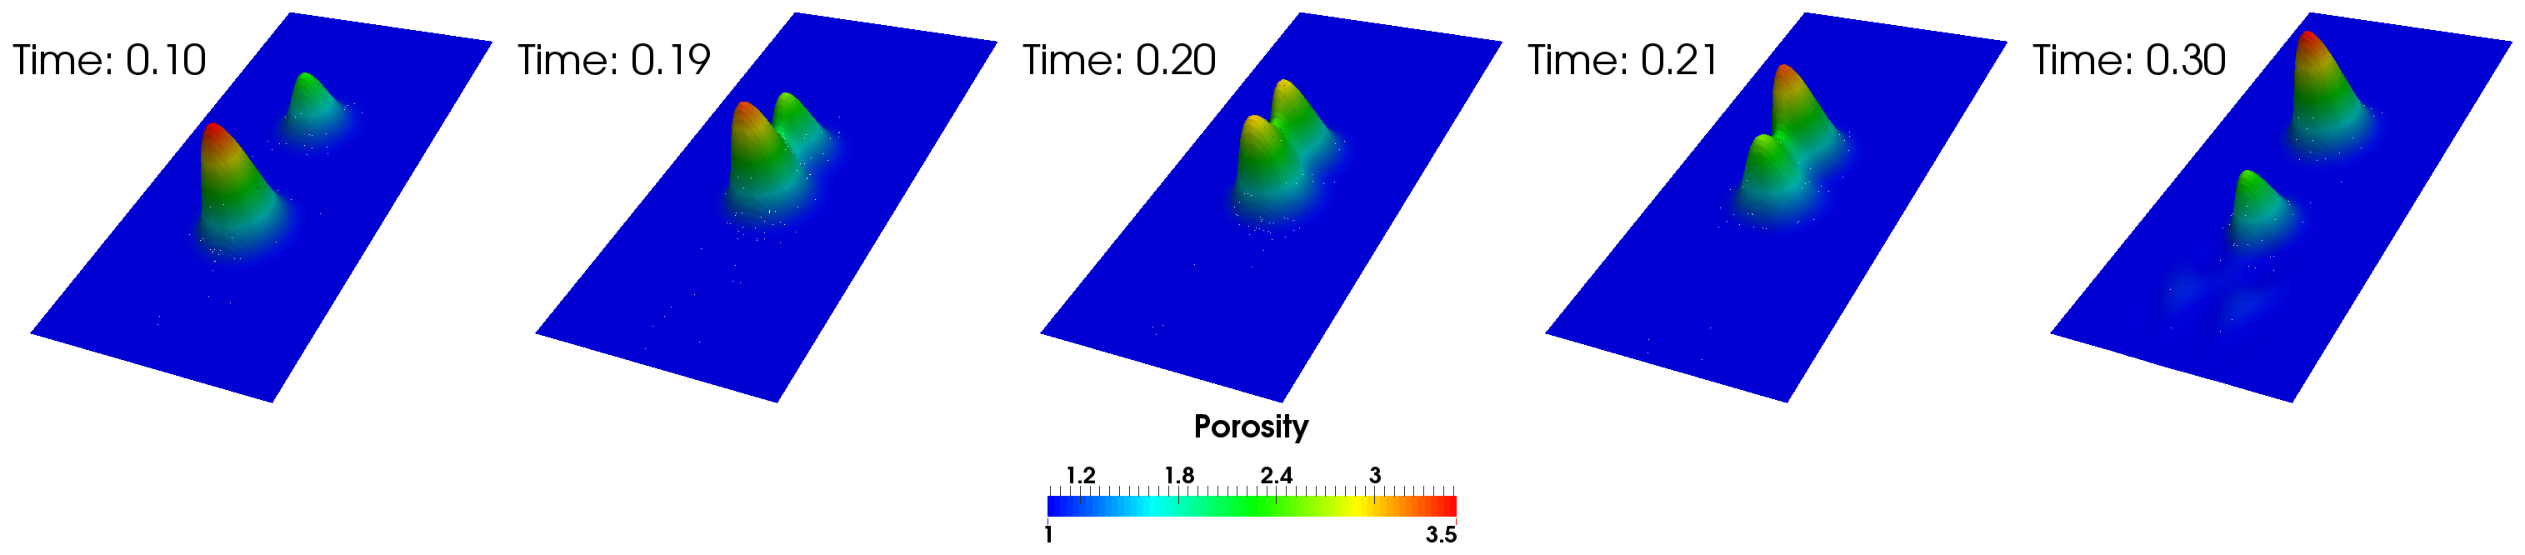
\includegraphics[width=\textwidth]{figures/collision.pdf}
  \caption{Non-linear collision of two 2-D solitary waves, the larger
    wave has a speed $c=7$ which collides with a smaller wave with
    $c=5$. This calculation is done in a frame moving at the mean
    velocity of the two solitary waves (i.e. $W=-6$).  While these
    porosity waves are not solitons (i.e. they are not completely
    conserved on collision), they do demonstrate a soliton-like
    collision property where there is a phase-shift in which  the large
    wave ``fills'' the smaller wave such that the two waves appear to
    trade places and then continue to propagate with unchanging form.
  Closer inspection of this model, though, shows the generation of a
  small amount of background porosity that is shed during the
  collision.  More oblique collisions produce more scattering of the
  porosity.  }
  \label{fig:collision}
\end{figure}

Another set of problems involve the interaction of multiple solitary
waves.  In the early days of magma dynamics where most calculations
were 1-D,  numerical solutions suggested that the collision of two
solitary waves showed soliton-like behavior where the two waves passed
through each other without scattering and the waves were often
referred to as magma solitons (or ``magmons'').  However it was soon
shown that even in 1-D the governing equations did not demonstrate an
infinite number of conservation laws and in fact showed scattering on
collision
\cite{barcilon_nonlinear-waves_1986,barcilon_solitary_1989}. Moreover,
in 2-D the scattering was much more noticeable. Figure
\ref{fig:collision} shows such a calculation done using \TF{} and a
fully worked out example for this model can be found in
\texttt{\$TF\_HOME/share/terraferma/tutorials/porositywaves/collision/magmawaves.tfml} 

Setting up such collision problems is relatively easy in \TF{} and
only requires minor modifications to the instability problem.  The
chief changes are
\begin{itemize}
\item Changing unit square to a rectangle such that
  $\Omega=[0.,0.5]\times[0.,1.]$
\item Change the porosity initial condition and coefficients to allow
  for two solitary waves and then take the maximum value of the two
  waves.  In particular,  the two waves will now have different speeds $c$
  and different initial locations $x_{0}$.  So we will need to
  \begin{itemize}
  \item add or modify the coefficients to include ones with names
    \texttt{c0},\texttt{x0} and \texttt{c1},\texttt{x1}.  The example
    uses \texttt{c0=7}, \texttt{x0=[ 0.25,0.25]}, \texttt{c1=5}, \texttt{x1=[0.25,0.75]}
  \item Modify the python for the initial conditions so that
    \texttt{TFSolitaryWave} knows about the new names.  The python in
    the example code is
    \begin{lstlisting}[style=python]
# Initialize to two solitary wave profiles 
# using PySolwave routines 
# This header will act as a global header to all subsequent def val instances
# (with great power comes great responsibility)

from pysolwave.tfsolitarywave import TFSolitaryWave
from glob import glob

tfmlfile = glob("magmawaves.tfml")[0]

#initialize solitary wave objects from tfmlfile
tfswave0 = TFSolitaryWave(tfmlfile,c_name="c0",x0_name="x0")
tfswave1 = TFSolitaryWave(tfmlfile,c_name="c1",x0_name="x1")

# print some diagnostics
print 'rmax = ',tfswave0.rmax, tfswave1.rmax
print 'c0,c1 =', tfswave0.swave.c, tfswave1.swave.c
print 'x0,x1 =', tfswave0.x0, tfswave1.x0

# python function for setting initial condition
import numpy as np
def val(x):
  global np,tfswave0,tfswave1
  xa = np.array(x)
  f0 = tfswave0.eval(xa)
  f1 = tfswave1.eval(xa)
  return max(f0,f1)
    \end{lstlisting}

  \end{itemize}
\item Change the run time and visualization dump period to adequately
  capture the collision. Here we only run to a dimensionless \texttt{finish\_time}
  of 0.5 visualizing every 0.01 time units.
\end{itemize}

Again, these time-dependent problems can take some time to run so the
example testharness file assumes two processors and runs in parallel.
It is straightforward to modify this file to explore other wave
combinations and different initial positions.  Have fun.

%%% Local Variables: 
%%% mode: latex
%%% TeX-master: "tftutorials"
%%% End: 
